\chapter{Toteutus}
\label{ch:toteutus}
Tässä osiossa käydään läpi kappaleessa \ref{ch:suunnittelu} suuniteltun ohjelman toteuttaminen. Toteutus alkaa yleiskuvalla sen komponenteista ja niiden toiminnasta. Yleiskuvan jälkeen pureudutaan ohjelman yksityiskohtiin kuten kirjastoihin ja niiden toimintaan. Lopuksi mietitään jatkokehitysideoita mitä olisi voinut lisätä, tehdä toisin ja mahdollisia puutteita.


\section{Yleiskuva}
\label{ch:rcb-sub-yleiskuva}
Työssä toteutetiin komentorivipohjainen ohjelma C-kielellä. Ohjelman tarkoitus oli tilata IED-laitteen viestit ja prosessoida ne JSON-muotoon RabbitMQ-palvelimelle. RabbitMQ:lta muut ohjelmat pystyivät tilaamaan JSON-viestejä. Kuvassa \ref{fig:rcb-sub-komponenttikaavio} on esitetty komponenttikaavio  toteutetusta ohjelmasta ja siihen käytetyistä kirjastoista. Toteutettu komponentti on kuvassa keskellä keltaisella ja nimelään rcb\_sub. Kuvasta voi nähdä miten eri komponentit ovat relaatiossa keskenään rcb\_sub-ohjelman kanssa. Kuvassa on myös esitetty IED-laite ja RabbitMQ-palvelin.

\begin{figure}[ht!]
	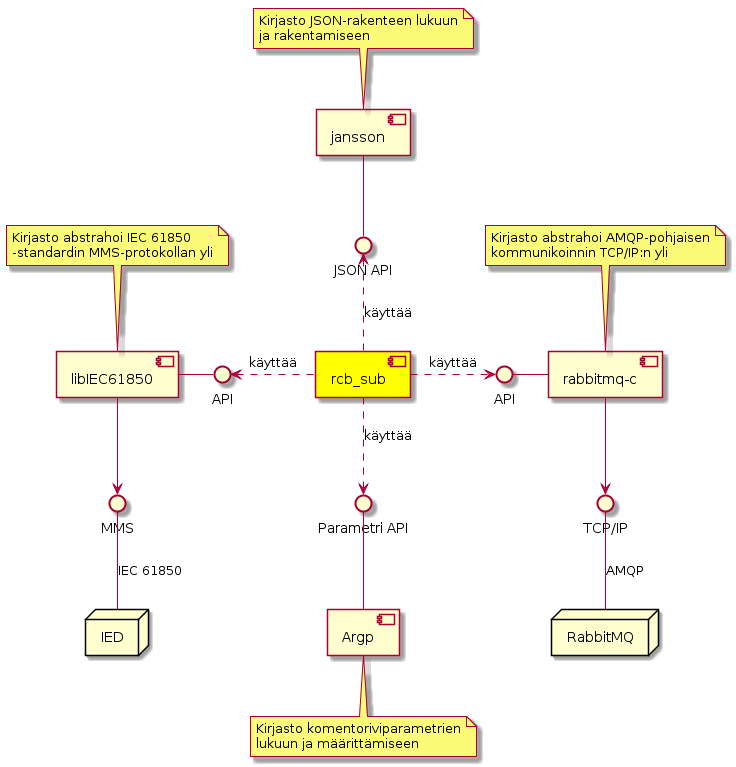
\includegraphics[width=1\textwidth]{pictures/rcb-sub-component-diagram.png}
	\caption{Toteutuksen komponenttikaavio sen osista ja relaatioista toisiinsa.}
	\label{fig:rcb-sub-komponenttikaavio}
\end{figure}

Toteutuksessa käytettiin seuraavia kirjastoja:
\begin{itemize}
	\item libiec61850,
	\item rabbitmq-c,
	\item jansson, ja
	\item Argp.
\end{itemize}
Kaikki käytetyt kirjastot on toteutettu C-kielellä, kuten rcb\_sub. Kirjastojen tarkoitus on abstrahoida jonkin asian käyttö ja tarjota käyttäjälle siitä helppokäyttöinen ja ymmärrettävä rajapinta. Rajapintaa käyttämällä kirjasto hoitaa matalan tason toiminnan ilman että kirjaston käyttäjän tarvitsee siitä välittää. Kirjasto libiec61850 abstrahoi IEC 61850 -standardin käyttöä ja hoitaa matalan tason MMS-protokollan kommunikoinnin \cite{libIEC61850-repo}. Samaa kirjastoa käytettiin ensimmäisessä demoversiossa (kappale \ref{ch:demoversio-ja-sen-toiminta}) ja kirjaston kerrosarkkitehtuuri oli esitetty kuvassa \ref{fig:libiec61850-layer-architecture}. Kuvassa \ref{fig:rcb-sub-komponenttikaavio} libiec61850 kommunikoi suoraan IED-laitteen kanssa MMS-protokollan yli. Kirjasto rabbitmq-c abstrahoi RabbitMQ-palvelimen käyttöä ja hoitaa matalan tason AMQP-pohjaisen kommunikoinnin \cite{rabbitmq-c-repo}. Toteutuksessa rabbitmq-c kommunikoi suoraan RabbitMQ-palvelimen kanssa. Kirjasto jansson abstrahoi JSON-rakenteiden lukua ja käsittelyä C-kielelle \cite{jansson-repo}. Kirjastoa käytettiin rakentamaan IED-laitteelta tulleesta viestistä JSON-muotoinen viesti. JSON-rakenne on nähtävissä liitteessä \ref{ch:report-json-format}. Kirjasto Argp auttaa ohjelman komentoriviparametrien määrittämisessä ja käsittelyssä \cite{argp-glibc-guide}. Kirjasto auttaa toteuttamaan ohjelmalle UNIX-tyyliset parametrit. Eli vaaditut parametrit ja vaihtoehtoiset lyhyet ja pitkä parametrit. Vaadituista parametreista esimerkiksi Linux:in komento \texttt{mv foo.txt bar.txt}, jossa foo.txt ja bar.txt ovat vaadittuja parametreja. Vaihtoehtoisista parametreista esimerkkinä pitkä muoto \texttt{-{}-bytes} ja lyhyt muoto \texttt{-b}. Lisäksi kirjasto lisää ohjelmaan automaattisesti Linux:ista käyttäjille tutut \texttt{-{}-help} ja \texttt{-{}-version} vaihtoehtoiset parametrit. Kommennolla \texttt{-{}-help} kirjasto tulostaa Linux:ilta tutun ohjelman aputeksin käyttäjälle, jossa on esitettu ohjelman kaikki parametrit ja niiden selitteet \cite{step-by-step-into-argp}.

Kuvassa \ref{fig:rcb-sub-sekvenssikaavio} on esitetty rcb\_sub-ohjelman sekvenssikaavio pääpiirteisestä toiminnasta. Toteutus noudattaa suurinpiirtein samoja periaatteita kuin demototeutus (kuva \ref{fig:sequence-diagram-report-subscription}). Tässä käydään läpi ohjelman pääpiirteinen toiminta ja sitä käydään tarkemmin läpi kappaleessa \ref{rcb-sub-toiminta}. Ensin ohjelman toiminta alkaa lukemalla ja annetut parametrit Argp-kirjastolla. Parametreissa tulee tiedot yhteyden muodostamiseen IED-laitteelle ja RabbitMQ-palvelimelle. Parametreissa on myös tiedot RCB-instansseista jotka halutaan IED:ltä tilata. Yhteyksien muodostamisen jälkeen jokainen parametrina annettu RCB käydään läpi silmukassa ja sen arvot ja datajoukon viitteet luetaan IED:ltä. Tämän jälkeen sisäkkäisessä silmukassa luetaan datajoukon viitteiden muuttujien spesifikaatiot (kohdat 11--12). Spesifikaatio antaa tiedot muuttujien pituudesta ja tyypistä. Näitä tietoja käytetään JSON-rakenteessa (esimerkkinä liiteessä \ref{ch:report-json-format} rivit 21--22). Tämän jälkeen tehdään toinen silmukka jossa jokainen RCB-instanssi tilataan ja niille asetetaan takaisinkutsufunktio (kohdat 13--16). Arvojen kirjoitushetkellä (kohta 15) RCB varataan ja se aloittaa viestien lähettämisen rcb\_sub-ohjelmalle. Jokaisen RCB:n kirjoituksen jälkeen ohjelma jää loputtomaan silmukkaan ja jää odottamaan viestejä vastaan. Viestin saapuessa asetettua takaisinkutsufunktiota kutsutaan ja jonka parametrina on saapunut viesti (kohta 17). Viesti muutetaan JSON-muotoon jansson-kirjastolla ja julkaistaan RabbitMQ-palvelimelle rabbitmq-c-kirjastolla (kohdat 17--22).

\begin{figure}[ht!]
	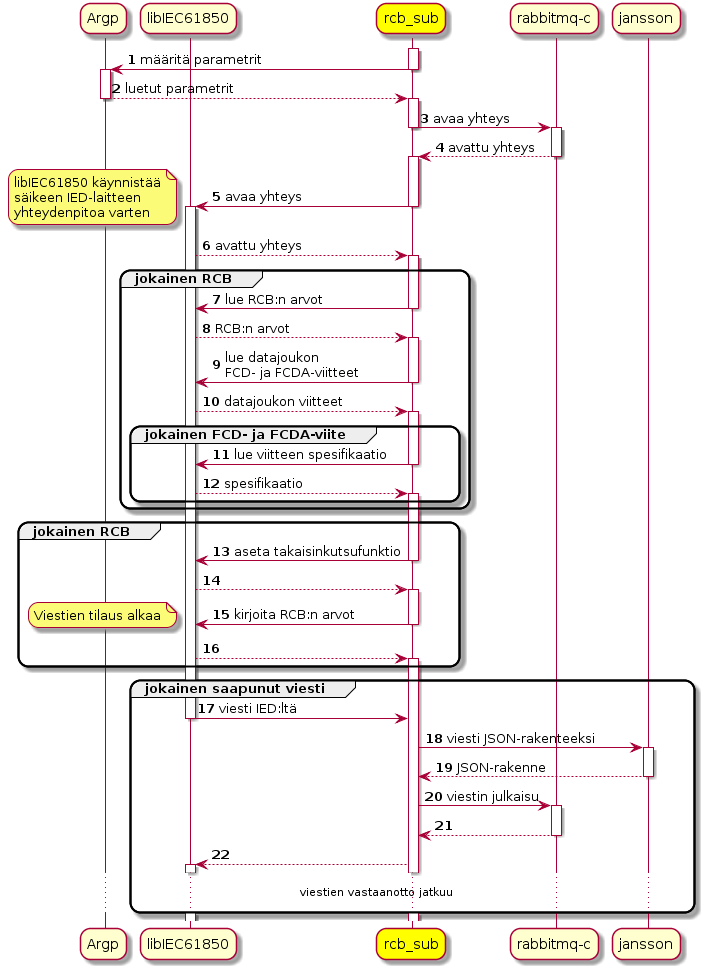
\includegraphics[width=1\textwidth]{pictures/rcb-sub-general-sd.png}
	\caption{Sekvenssikaatio rcb\_sub-ohjelman kokonaistoiminnasta.}
	\label{fig:rcb-sub-sekvenssikaavio}
\end{figure}


\section{Ohjelman toiminta}
\label{rcb-sub-toiminta}
Tulevissa kappaleissa käydään läpi yksityiskohtaisemmin rcb\_sub-ohjelman toimintaa, joka esiteltiin pääpiirteittäin kappaleessa \ref{ch:rcb-sub-yleiskuva}. Kappaleiden järjestys noudattaa kuvassa \ref{fig:rcb-sub-sekvenssikaavio} olevan sekvenssikaavion järjestystä. Toisin sanoen ohjelmaa käydään läpi tarkemmin siinä järjestyksessä jossa sen suoritus tapahtuu.


\subsection{Parametrisointi}
Ohjelma parametrisoitiin Argp-kirjastolla. Kirjasto tarjoaa rajapinnan komentoriviparametrien käsittelyyn ja määrittämiseen. Parametrien muodot ovat tuttut muista Linux-käyttöjärjestelmän parametreista ja samaa periaatetta käytettiin tässäkin ohjelmassa. Kirjasto myös lisäsi ohjelmaan automaattisesti aputekstin käyttäjää varten. Aputeksti sisältää tietoa ohjelman parametreista ja niiden selitteistä. Aputekstin pystyi ohjelmsata tulostamaan parametrilla \texttt{-{}-help}. Liitteessä \ref{ch:rcb-sub-help-output} on esitetty miltä toteutetun ohjelman aputeksti näyttyy. Liitteestä voi myös nähdä kaikki ohjelman käytettävät parametrit ja lyhyen selityksen mihin ja kuinka sitä käytetään.

Ohjelmiston parametrit voidaan ajatella koostuvan kolmesta eri ryhmästä. Ensin päätason vaihtoehtoiset parametrit \texttt{OPTIONS}. Pakolliset parametrit \texttt{EXCHANGE} ja \texttt{ROUTING\_KEY}. Viimeisenä n-kappaletta \texttt{RCB\_REF} ja \texttt{RCB\_OPTIONS} parametreja. Suurin osa \texttt{OPTION} parametreista on itsestäänselviä. Esimerkkinä \texttt{-{}-amqp-host}, joka kertoo AMQP-palvelimen IP-osoitteen. Tai \texttt{-{}-ied-host}, joka kertoo IED-laitteen IP-osoitteen johon yhdistetään. Parametrit \texttt{EXCHANGE} ja \texttt{ROUTING\_KEY} määrittävät nimet RabbitMQ-palvelimen vaihteelle ja reititysavaimelle. \texttt{RCB\_REF} määrittää viitteen tilattavaan RCB-instanssiin IED-laitteella. Tätä seuraava vaihtoehtoinen \texttt{RCB\_OPTIONS} määrittää parametrit edeltävälle RCB-instanssille, millä instanssi konfiguroidaan ennen tilausta. RCB-instansin parametri \texttt{RCB\_OPTIONS} määrittää käytetyt vaihtoehtoiset kentät (\texttt{-{}-opt-fields}), käytetyt liipaisimet (\texttt{-{}-trigger}) ja pyydetäänkö yleistä kyselyä ennen muita viestejä (\texttt{-{}-gi}). Liipaisimet ja vaihtoehtoiset kentät asetetaan numeerisella arvolla, jotka löytyvät myös aputekstistä (liite \ref{ch:rcb-sub-help-output}). Numeerisia arvoja voidaan summata yhteen asettamalla monta arvoa yhtä aikaa.

\subsection{Yhteyksien muodostus}


\subsection{IED:n attribuuttien määritysten luku}


\subsection{Viestien tilaus}


\subsection{JSON:nin muodostaminen}


\section{Jatkokehitys}
\begin{it}
	Kirjoita tähän ideoita mitä jää jatkokehitykseen ja mitä ohjelmistossa on puutteita tai mitä jäi tekemättä. Esim. testaus ja CMake lisääminen.
\end{it}